%! Author = javad
%! Date = 04/01/2024

\subsection{Legibility Score}

The original formula for motion legibility (by Dragan et al. \cite{dragan2013legibility}) for an observed trajectory $\xi$ \cite{dragan2013legibility} is as follows:

\begin{equation}
    \label{eq_dragan9}
    \text { legibility }(\xi)=\frac{\int P\left(G^* \mid \xi_{S \rightarrow \xi(t)}\right) f(t) d t}{\int f(t) d t}
\end{equation}

\noindent
This equation assumes $P\left(G \mid \xi_{S \rightarrow \xi(t)}\right)$ is the way an observer distributes probabilities to potential goals of the robot, with $G^*$ being the true goal of the robot, and $f(t)$ to be a descending function like $f(t)=T-t$ which assigns higher weights to the initial parts of the trajectory, justifying the fact that a legible motion should minimize the ambiguity as soon as possible for the observers.

\noindent
To compute Eq. (\ref{eq_dragan9}), they use the Bayse' rule and rewrite $P\left(G^* \mid \xi_{S \rightarrow \xi(t)}\right)$ as below:

\begin{equation}
    \label{eq_dragan8}
    P\left(G \mid \xi_{S \rightarrow Q}\right) \propto \frac{\exp \left(-C\left(\xi_{S \rightarrow Q}\right)-C\left(\xi_{Q \rightarrow G}^*\right)\right)}{\exp \left(-C\left(\xi_{S \rightarrow G}^*\right)\right)} P(G)
\end{equation}

\noindent
with $P(G)$ being a prior distribution of the potential goals and $C(\xi)$ being a cost function for an observed trajectory $\xi$ or an optimal trajectory $\xi^*$.
%In the original work of Dragan et al. \cite{dragan2013legibility} however, this is considered as a Euclidean distance between the initial and the goal point for the latter,
%which makes it too simplistic, i.e. a real human might use his own knowledge and reasoning for predicting the robot's goal based what they observe and making this simple assumption is not always aligned with human actualities.


% \begin{figure}
%     \centering
%     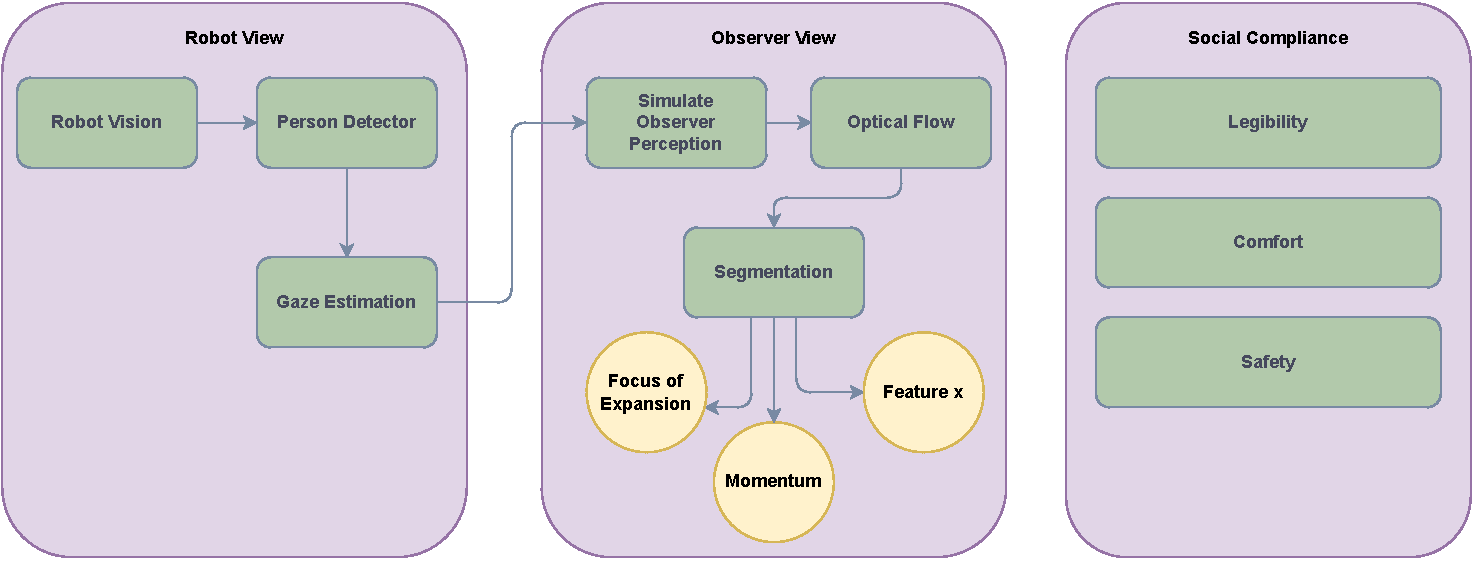
\includegraphics[width=0.8\textwidth]{figs/Legibot-fig1.pdf}
%     \caption{Overview}
%     \label{fig:enter-label}
% \end{figure}
